\chapter{不确定环境下安全约束方法}

在不确定环境中，机器人自主决策不仅需要完成目标导航、避障或任务执行等基本功能，还需要在感知误差和环境变化等因素影响下保持稳定的安全行为。
传统强化学习方法通常通过奖励惩罚引导策略避免危险状态，但这类软约束方式难以保证训练与部署过程中始终满足硬安全约束；
同时，机器人系统的运动学限制和状态估计误差也会进一步放大策略执行中的碰撞风险。

针对上述问题，本章围绕不确定环境下的安全强化学习展开研究，提出一种基于约束流形的安全策略学习方法。
该方法将安全约束显式嵌入策略执行过程，通过约束流形投影对策略动作进行实时修正，并结合离线安全可达性分析与数据驱动状态估计机制，提高策略在复杂环境中的安全性和鲁棒性。

% 针对机器人在强安全约束环境中进行强化学习训练时须严格遵循硬安全约束的问题，
% 同时优化感知不确定性以及安全约束高度依赖先验模型的问题，本文提出了一种基于约束流形的安全空间过滤框架。
% 利用系统可达性分析为，从离线轨迹数据中预先计算环境感知的安全区域，
% 在部署阶段无需实时感知即可自适应调节安全裕度，从而为机器人提供具有物理意义的安全边界描述。
% 同时引入流形安全过滤与校准机制，通过零空间投影（Null-space Projection）将策略动作投影至约束流形的切空间上，
% 并结合奖励校准机制引导策略学习内在的安全行为，使得策略更新始终满足硬安全约束要求。
% 针对实际机器人系统中普遍存在的传感器噪声与定位误差问题，本文进一步引入数据驱动的扩展卡尔曼滤波（EKF），
% 利用卷积神经网络（CNN）学习噪声参数，使测量协方差能够适应与速度相关的传感器噪声，
% 对机器人自身状态进行更加精确和鲁棒的估计，从而显著降低了因感知不确定性引发的安全风险。
\section{问题定义}
为刻画机器人安全导航中的安全关系，考虑一个机器人在包含 $n$ 个障碍物的复杂环境中进行导航任务。令 $s_t = [p_t^\top, v_t^\top]^\top \in \mathcal{S} \subseteq \mathbb{R}^d$ 表示机器人在离散时间步 $t$ 时的状态，其中 $p_t \in \mathbb{R}^{d_p}$ 代表位置向量，$v_t \in \mathbb{R}^{d_p}$ 代表速度向量（$d_p$ 通常为 2 或 3）。为了定量描述安全，引入基于距离的约束函数。安全性的核心要求是机器人与环境中任何障碍物之间必须保持一定的物理间隔。定义约束集合如下：$$c_i(s_t) := d_{\text{safe}} - \|p_t - o_i\|_2 \leq 0, \quad \forall i \in \{1, \ldots, n\}$$其中，$d_{\text{safe}} > 0$ 表示预设的最小安全距离阈值，$o_i \in \mathbb{R}^{d_p}$ 为第 $i$ 个障碍物在空间中的坐标，$\|\cdot\|_2$ 为欧几里得范数。

若状态 $s_t$ 满足对所有 $i$ 均有 $c_i(s_t) \leq 0$，则称该状态是安全的。在物理上意味着机器人的中心与所有障碍物的中心的距离均大于等于 $d_{\text{safe}}$。在实际应用中，该距离通常考虑了机器人自身的几何半径以及感知系统的不确定性冗余。

在强化学习（RL）框架下，将安全导航任务建模为一个约束马尔可夫决策过程（CMDP），记为六元组 $(\mathcal{S}, \mathcal{A}, P, R, \gamma, C)$。其中：$\mathcal{S}$ 和 $\mathcal{A}$ 分别为状态空间和动作空间；$P: \mathcal{S} \times \mathcal{A} \times \mathcal{S} \rightarrow [0, 1]$ 为环境的状态转移概率核；$R: \mathcal{S} \times \mathcal{A} \rightarrow \mathbb{R}$ 为奖励函数，鼓励机器人靠近目标点；$\gamma \in [0, 1)$ 为折扣因子；$C = \{c_i: \mathcal{S} \rightarrow \mathbb{R}\}_{i=1}^k$ 为与环境障碍物对应的约束集合。在具有 $k=n$ 个硬约束（每个障碍物对应一个约束）的设置下，安全强化学习的目标是寻找到一个最优策略 $\pi: \mathcal{S} \rightarrow \mathcal{A}$，使得在满足所有时间步的硬安全约束前提下，最大化累积期望回报：$$\max_{\pi} \mathbb{E}_{\pi}\left[ \sum_{t=0}^{T} \gamma^t R(s_t, a_t) \right]$$$$\text{s.t. } c_i(s_t) \leq 0, \quad \forall t \in \{0, \dots, T\}, \forall i \in \{1, \dots, n\}$$与传统的强化学习不同，CMDP 要求算法在探索过程中不仅要学习任务技能，还必须严格遵守状态空间的边界，避免任何形式的碰撞。

此外，考虑到机器人系统（如差速驱动轮式机器人或无人机）普遍存在非完整约束（Nonholonomic Constraints），不能简单地假设状态可以任意改变。因此，本文将机器人的底层运动学建模为连续时间的控制仿射系统（Control-Affine System）：$$\dot{s} = f(s) + G(s) a$$

在该模型中：$a \in \mathcal{A} \subseteq \mathbb{R}^m$ 是 $m$ 维控制控制量（如推力、转矩或速度指令）；$f(s): \mathcal{S} \rightarrow \mathbb{R}^d$ 称为漂移项（Drift term），代表系统在无控制输入时的固有动力学演化；$G(s): \mathcal{S} \rightarrow \mathbb{R}^{d \times m}$ 为控制输入矩阵，定义了控制动作如何映射到状态的变化率上。动力学特例：质点模型（Single-Integrator）： 若 $f(s) = 0$ 且 $G(s) = I$，系统简化为全向移动模型。差速驱动模型： $G(s)$ 包含三角函数项（如 $\cos\theta, \sin\theta$），用以体现机器人朝向与运动速度之间的耦合关系。通过结合上述动力学模型与 CMDP 框架，本文的研究重点在于如何在复杂的动力学约束下，保证机器人在轨迹执行过程中的实时安全性。

\section{约束流形策略学习方法}
本文构建了一种面向安全强化学习的约束流形策略方法（Constrained Manifold Policy Learning，CMPL），通过约束流形建模、可达性分析与状态估计的协同设计，实现策略安全性。整体框架由以下三个核心模块组成：
\begin{itemize}
\item \textbf{基于约束流形的安全过滤器}：
针对策略输出可能违反安全约束的问题，本文设计基于零空间投影的动作修正机制，将名义动作投影至约束流形的切空间，从而保证生成动作始终满足硬约束。在此基础上，引入动态奖励校准机制，对动作修正幅度进行显式调节，使策略在训练过程中逐步适应约束结构，形成内生的安全行为，而非单纯依赖外部惩罚项。

\item \textbf{离线安全可达空间构建}：  
为提升系统对环境约束的感知能力，本文引入可达性分析方法，在离线阶段基于采样轨迹与环境先验信息预计算安全可达区域。所得可行性值函数在部署时用于动态调节安全裕度，使系统在无需实时精确建模障碍物的情况下，仍能保持保守且稳定的安全行为。

\item \textbf{数据驱动的状态估计模块}：  
为缓解感知噪声对安全决策的影响，本文构建基于数据驱动的扩展卡尔曼滤波（EKF）框架，通过卷积神经网络学习观测噪声参数，使测量协方差能够随运动状态自适应调整，从而在速度相关噪声条件下维持较高的状态估计精度，保证安全过滤器输入的可靠性。
\end{itemize}

在具体实现中，可达性分析与状态估计模块均采用离线构建方式。前者利用环境数据提前学习安全裕度分布，后者根据交互数据刻画传感器噪声随运动状态变化的特征。部署阶段，系统只需调用已经得到的安全边界和噪声估计结果，无需重新进行在线训练或复杂优化。这样的设计降低了运行时计算开销，也提高了方法在资源受限机器人平台上的部署可行性。

\begin{figure}
    \centering
    
\includegraphics[width=1\linewidth]{images/framework.png}
    \caption{约束流形策略学习方法框架}
    \label{fig:placeholder}
\end{figure}
\subsection{约束流形投影}
流形是一个局部与欧几里得空间同胚的拓扑空间， 可以用于描述复杂的几何对象，例如曲线、曲面以及更高维的结构。约束流形是由某些约束条件定义的流形，这些约束条件限制系统的状态或行为。在几何上，这些约束可以用方程或不等式来描述。
\subsubsection{（1）松弛变量}
然而，不等式约束在优化和控制律设计中往往难以直接处理，且难以定义稳定的切空间（Tangent Space）。为此，本研究引入非负松弛变量（Slack Variables） $\mu \in \mathbb{R}^k_{\geq 0}$。通过将原始约束函数与松弛变量结合，可以将不等式约束转化为严格的等式约束形式：
\begin{equation}
    \bar{c}(s, \mu) := c(s) + \mu = 0, \quad \text{其中 } \mu \geq 0\label{eq:slack}
\end{equation}

引入松弛变量后，由于 $\mu$ 被限制为非负，任何满足等式 $\bar{c}(s, \mu) = 0$ 的点都必然满足 $c(s) = -\mu \leq 0$，安全性得到了自然的保证。这种转化允许将安全状态的搜索范围从一个区域（区域约束）缩小到一个精确定义的数学流形上。基于此，本文定义约束流形 $\mathcal{M}$ 为满足所有安全准则的状态集合：
\begin{equation}
    \mathcal{M} := { (s, \mu) \in \mathcal{D} \mid \bar{c}(s, \mu) = 0 
}\end{equation}

其中 $\mathcal{D} = \mathcal{S} \times \mathbb{R}^k_{\geq 0}$ 代表由原始状态与松弛变量构成的增广状态空间（Augmented State Space）。

\subsubsection{（2）零空间投影}
设$a_{\text{unsafe}} \in \mathbb{R}^m$表示由强化学习策略输出的未受约束的动作（unconstrained action）。
为了保证系统在执行控制输入时始终满足安全约束，安全过滤器首先在内部构造一个增广参考向量：
$u_{\text{ref}} =
\begin{bmatrix}
a_{\text{unsafe}}^\top , \mathbf{0}^\top
\end{bmatrix}^\top
\in \mathbb{R}^{m+k}$
其中 $k$ 表示约束数量（对应引入的松弛变量）。安全过滤器随后将该参考向量转换为满足所有约束条件的安全控制量：
$\begin{bmatrix}
a_{\text{safe}}^\top , \dot{\mu}^\top
\end{bmatrix}^\top$
其中 $a_{\text{safe}}$ 为最终执行的安全动作，$\dot{\mu}$ 为松弛变量的变化率。通过这种方式，可以在尽量保持策略原始控制意图的同时，保证系统始终处于安全可行域内。

对约束函数取时间导数可得：
\begin{equation}
\frac{d}{dt} \bar{c}(s, \mu) = J_s \dot{s} + J_\mu \dot{\mu} = J_s f(s) + J_c
\begin{bmatrix}
a \
\dot{\mu}
\end{bmatrix}
\label{eq:constraint_deriv}
\end{equation}

其中
$J_s = \frac{\partial \bar{c}}{\partial s},\quad
J_\mu = \frac{\partial \bar{c}}{\partial \mu}$
分别表示约束函数关于状态变量和松弛变量的雅可比矩阵。定义组合约束雅可比矩阵$J_c = [J_s G(s), J_\mu] \in \mathbb{R}^{k \times (m+k)}$ 刻画了控制输入与松弛变量对约束变化率的整体影响。

为了使系统状态始终保持在约束流形上，需要满足$\frac{d}{dt}\bar{c} = 0$ ，即系统的状态变化始终位于约束流形的切空间中。设 $J_c^\dagger$为为矩阵 $J_c$ 的 Moore--Penrose 伪逆，定义零空间投影算子：
\begin{equation}
N_c = I - J_c^\dagger J_c
\end{equation}

该投影矩阵将任意向量投影到 $J_c$ 的零空间，从而保证控制输入不会破坏约束条件。
则安全动作通过以下公式计算：
\begin{equation}
\begin{bmatrix}
a_{\text{safe}} \
\dot{\mu}
\end{bmatrix}
=
N_c u_{\text{ref}}
-
J_c^\dagger
\bigl(
J_s f(s) + K_c \bar{c}(s, \mu)
\bigr)
\label{eq:safe_action}
\end{equation}

其中 $K_c > 0$ 为约束修正增益。公式中的第一项将增广参考向量投影到约束零空间（即约束流形的切空间），从而保证生成的控制输入不会导致约束违反；第二项同时补偿系统漂移动力学 $f(s)$，并驱动系统状态逐渐回到约束流形上，从而保持系统在安全集合内演化。

\begin{theorem}[安全性保证]
\label{thm:safety}

假设约束雅可比矩阵 $J_c$ 在系统轨迹上始终具有满行秩。若系统初始状态满足约束流形条件，即
$\bar{c}(s_0, \mu_0) = 0$
且 $\mu_0 \geq 0$，并且控制输入按照公式~\eqref{eq:safe_action} 进行计算，则对于任意时间 $t \geq 0$，系统始终满足$c(s_t) \leq 0$即系统始终保持安全。
\end{theorem}

\begin{proof}
\renewcommand{\qedsymbol}{}%
由于 $J_c$ 满行秩，有$J_c J_c^\dagger = I_k$且$J_c N_c = 0$，将控制律~\eqref{eq:safe_action} 代入约束导数公式~\eqref{eq:constraint_deriv}：
\begin{align*}
\dot{\bar{c}} &= J_s f(s) + J_c \bigl[ N_c , u_{\text{ref}} - J_c^\dagger (J_s f(s) + K_c \bar{c}) \bigr] \\
&= J_s f(s) - J_c J_c^\dagger J_s f(s) - K_c J_c J_c^\dagger \bar{c} \\
&= J_s f(s) - J_s f(s) - K_c \bar{c} \\
&= -K_c \bar{c}
\end{align*}

当初始条件满足$\bar{c}(0) = 0$时，该微分方程的唯一解为$\bar{c}(t) = 0$
对所有 $t \ge 0$ 成立。由于投影操作保证 $\mu(t) \ge 0$，因此
\[c(s_t) = \bar{c}(t) - \mu(t) = -\mu(t) \le 0\]
从而系统始终满足安全约束。
\end{proof}

\textbf{说明（具体实施）.} 在实际实现中，为了提高数值稳定性，本文采用阻尼伪逆（damped pseudoinverse）
\[
\hat{J}_c^\dagger = J_c^\top (J_c J_c^\top + \epsilon I)^{-1}
\]

其中 $\epsilon > 0$ 为较小的正数。此时会引入残差$| J_c \hat{J}_c^+ - I_k | = O(\epsilon)$

因此理论上的严格不变性 $\bar{c}(t)=0$ 将变为
$\bar{c}(t) = O(\epsilon)$
即约束误差保持在一个小邻域内。同时修正项
$K_c \hat{J}_c^\dagger \bar{c}$
会持续将系统状态拉回约束流形，从而在 $\epsilon$ 足够小时仍能保持较低的约束违反程度。

\textbf{说明（离散时间）.} 在离散时间实现中，以时间步长 $\Delta t$ 应用公式~\eqref{eq:safe_action} 会引入每步
$O(\Delta t^2)$
的有界误差。结合修正项的作用，当 $\Delta t$ 相对于 $K_c$ 足够小时，系统仍能够维持约束满足，从而保证整体安全性。

\subsubsection{（3）奖励修正}
此外，本文优化了奖励修正方法。在强化学习中，惩罚约束违反是鼓励安全性的一种常见方法。通常的做法是在约束被违反时，向奖励中引入一个负常数惩罚项，但这种方法未考虑动作的不安全程度。当强化学习提出不安全的的动作时，安全流形过滤器会对其做出相应的的修正使其符合安全标准。而修正的幅度则量化了该动作的不安全程度。

因此，在奖励中引入一个与修正幅度相关的惩罚项，通过惩罚修正，可以更精细地控制系统的安全性。将这种奖励修正方法与安全流形过滤器结合使用，这种修改能够鼓励安全性并最小化修正。利用安全过滤器惩罚奖励的通用框架为：
\begin{equation}
    \begin{split}
        &R_{\alpha}(s_t,a_{{uncert},t},a_{safe,t}) \\
        &=R(s_t,a_{applied,t})-\alpha P(a_{uncert,t},a_{safe,t})
    \end{split}
\end{equation}

其中，$\alpha$ 是惩罚权重，$P$ 是基于修正的惩罚函数，$a_{applied,t}$是实际应用于系统的动作（在标准 RL 训练中为$a_{uncert,t}$ 而在过滤训练动作时为$a_{safe,t}$）。

\begin{algorithm}
\caption{Policy Iteration with Constraints}
\begin{algorithmic}[1]
\STATE \textbf{Input:} $c(s)$, parameters
\FOR{ $i=1$ \TO $N$ }
    \STATE Initialize feasible state $s_0$ and slack variable $\mu_0$
    \FOR{ $k=0$ \TO $T-1$ }
        \STATE Sample action $\alpha_k \sim \pi(\cdot \mid s_k)$
        \STATE Observe state $s_k$
        \STATE Compute $J_c(s_k,\mu_k)$, $N_c(s_k,\mu_k)$, and action $a_k$
        \STATE Apply action $a_k$
        \STATE Observe next state $s_{k+1}$ and reward $r_k$
        \STATE Provide the tuple $(s_k, a_k, s_{k+1}, r_k)$ to the RL
    \ENDFOR
\ENDFOR
\end{algorithmic}
\end{algorithm}

\subsection{安全可达性分析}
约束流形过滤器需要已知障碍物的位置，本文假设这些信息可以通过静态障碍物的先验地图获得（例如来自离线建图或仿真中的真实环境数据）。为了进一步构建能够自适应调节安全裕度的环境感知安全区域，本文采用离线HJ 可达性分析（Hamilton–Jacobi reachability analysis）。

\subsubsection{（1）从 HJ 偏微分方程到可行性值函数}
在连续时间系统中，给定约束函数 $c(s) \leq 0$ 定义安全集合
\begin{equation}
    \mathcal{K} = {s : c(s) \leq 0}
\end{equation}

以及系统动力学 $\dot{s} = f(s, a)$，HJ可达性分析将机器人状态分为可行状态和不可行状态，当机器人不存在满足硬约束的策略时，此时的状态被称为不可行状态，其余状态为可行状态。 可行区域则包含所有至少存在一个满足硬约束策略的可行状态。 

Hamilton–Jacobi 变分不等式（HJ-VI）刻画了后向可达管（Backward Reachable Tube, BRT）——即从某些初始状态出发，无论采取何种控制策略都无法避免最终违反约束的状态集合~\cite{bansal2017hj_reachability}：
\begin{equation}
\max\{c(s) - V(s), \min_{a} \nabla_s V(s)^\top f(s, a)\} = 0
\label{eq:hj_vi}
\end{equation}

以及零次水平集 ${s : V(s) \leq 0}$， 表示最大可行核（viability kernel）——即 $\mathcal{K}$ 中最大的受控不变子集。

对于离散时间系统 $s_{t+1} = f(s_t, a_t)$，HJ-VI~\eqref{eq:hj_vi} 可以化简为如下不动点方程：
\begin{equation}
    V(s) = \max{c(s), \min_a V(f(s,a))}
\end{equation}

据此定义对应的最佳可行状态值函数 $V^*_c$ 和最佳可行动作值函数 $Q^*_c$ 被定义为：
\begin{equation}
    V^*_c(s):=\min_{\pi}V^{\pi}_c(s):=\min_{\pi}\max_{y\in N}c(s_t) 
\end{equation}
\begin{equation}
    Q^*_c(s,a):=\min_{\pi}Q^{\pi}_c(s,a):=\min_{\pi} \max_{t\in \mathbb{N}}c(s_t).
\end{equation}

这里，$V^{\pi}_c(s)$表示策略 $\pi$ 从状态 $s$ 出发的轨迹中最大的约束违反值。如果$V^{\pi}_c(s) \leq 0$，说明策略 $\pi$ 能够满足从状态 $s$ 开始的硬约束。这意味着在所有的时间点 $t$ ，$c(s_t)\leq 0$ 。如果$V^*_c(s) \leq 0$，则存在至少一个策略 $\pi$ 能够满足状态 $s$ 开始的硬约束。可行价值函数表明策略是否能够满足硬约束（即策略的可行性）；而最优可行价值函数表示是否存在实现硬约束（即状态可行性）的策略。

对于策略 $\pi$ 的可行区域定义为 $S^{\pi}_f:=\{s|V^{\pi}_c(s) \leq 0\}$ ，即策略 $\pi$ 能够满足硬约束的状态集合。最大可行区域（viability kernel）定义为 $S^*_f:=\{s|V^*_c(s) \leq 0\}$ ，即包括所有存在至少一个满足硬约束策略的状态。 对于状态 $s$ ，可行策略集合定义为 $\Pi_{f(s)}:=\{\pi |V^{\pi}_c(s) \leq 0\}$ ，即包含所有从状态 出发能够满足硬约束的策略。

\subsubsection{（2）离线近似}
HJ 可达性分析在计算最优可行值函数需要通过与环境交互进行蒙特卡罗估计，这在离线设置中是不可行的。为了保证 Bellman 算子的收敛性，本文引入折扣因子 $\gamma \in (0, 1)$。通过反复利用带有折扣因子 $\gamma\to 1$的可行 Bellman 算子来获得近似的最优可行值。与 BRT 不动点对应的折扣可行 Bellman 算子定义为：
\begin{equation}
\mathcal{T}^* Q_c(s, a) := (1{-}\gamma) c(s) + \gamma \max{c(s), V_c(s')}
\label{eq:bellman}
\end{equation}

其中 $s' = f(s,a)$ 表示后继状态，而 $\max{c(s), \cdot}$ 对应于 HJ-VI~\eqref{eq:hj_vi} 中的 $\max$ 项：
该项确保值函数不会低于当前的约束违背程度，从而保持 BRT 的结构特性。

由于离线数据集无法全面覆盖所有的动作分布，因此在离线训练时可能出现数据集中未包含的动作。为了处理离线数据集 $\mathcal{D}$ 中的分布外动作，本文采用 expectile regression~\cite{kostrikov2022iql} 来近似 HJ-VI 中的 $\min_a$，而无需显式进行最小化：
\begin{align}
L_{V_c} &= \mathbb{E}*{(s,a) \sim \mathcal{D}} \left[ L^\tau*{\text{rev}}(Q_c(s,a) - V_c(s)) \right] \label{eq:loss_v} \\
L_{Q_c} &= \mathbb{E}_{(s,a,s') \sim \mathcal{D}} \left[ (\mathcal{T}^* Q_c - Q_c(s,a))^2 \right] \label{eq:loss_q}
\end{align}

其中$L^\tau_{\text{rev}}(u) = |\tau - \mathbf{1}(u > 0)| \cdot u^2$ ， $\tau \in [0.5, 1]$。该损失函数会对较小的 $Q_c$ 值赋予更高权重，从而偏向选择最安全（最乐观）的动作——这对应于 HJ-VI 中 $\min_a$ 的离散近似。

\subsubsection{（3）与安全过滤器的集成}
在部署阶段，学习得到的 $V^*_c$ 用于调节安全过滤器的保守程度。定义平滑权重函数：
\begin{equation}
    w(s) = \exp(V^*_c(s) / \delta)
\end{equation}

其中 $\delta > 0$ 为尺度参数，并据此调整危险半径：
\begin{equation}
d_{\text{danger}}(s) = d_0 + \eta  w(s)
\label{eq:danger_radius}
\end{equation}

其中 $d_0$ 为基础半径，$\eta > 0$ 控制安全裕度。

在可行区域内（$V^*_c \leq 0$），有 $w \in (0,1]$：
当状态接近边界（$V^*_c \approx 0$）时，$w \approx 1$，危险半径为 $d_0 + \eta$，即完整的扩展安全裕度；
当状态处于安全区域内部（$V^*_c \ll 0$）时，$w \approx 0$，危险半径约为 $d_0$，即接近名义安全距离。
对于不可行状态（$V^*_c > 0$），有 $w > 1$，此时系统会进一步增大安全裕度，从而提升保守性。

这种机制使得安全过滤器在部署阶段具备环境感知能力（environment-aware），而无需进行实时的障碍物检测或跟踪——预先计算得到的 $V^*_c$ 已经编码了来自先验地图的静态环境可达性结构。

% 通过离线交互数据训练后，可以获得一个可达安全动作值函数，用于预测在给定状态下执行某一动作是否会导致未来进入危险区域。由此获得一个连续、可微的安全判别函数，用于定义隐式安全约束边界。利用学习得到的安全动作值函数，在每个状态下定义安全可行动作集合。对于任意状态，该函数将动作空间划分为可执行的安全动作区域以及会导致未来危险的违规动作区域。由此，通过学习得到的值函数零水平面刻画的连续边界结，在状态–动作空间中形成安全流形。

\subsection{数据驱动的状态估计}
状态估计的精度会直接影响安全过滤器的判断结果。机器人在导航过程中通常依赖 GPS、视觉里程计等位置传感器获取状态信息，但这类测量并不稳定，噪声大小会随运行条件发生变化。以高速运动为例，机体振动、GPS 多路径效应以及视觉图像中的运动模糊都会更加明显，此时传感器观测误差往往高于低速运动状态。本文将这种与速度相关（velocity-dependent）的测量不确定性表示为：
\begin{equation}
\sigma(v) = \sigma_{\text{base}}(1 + k |v|)
\label{eq:vel_noise}
\end{equation}

其中，$\sigma_{\text{base}}$ 为基础噪声标准差，$k > 0$ 表示速度缩放系数，$|v|$ 表示机器人当前运动速度。常规 EKF 一般采用固定测量噪声协方差 $R = \sigma_{\text{base}}^2 I$，这种设定在低速或噪声较稳定的情况下较为方便，但当机器人速度较高时，这种固定协方差模型往往会过度信任噪声较大的测量数据，从而降低状态估计精度。基于此，本文采用一种数据驱动的扩展卡尔曼滤波方法，利用最近时间段的 IMU 测量数据预测当前测量噪声协方差，使滤波过程能够随运动状态变化进行调整。

\subsubsection{（1）扩展卡尔曼滤波}
本文采用扩展卡尔曼滤波（EKF）对非线性系统动力学进行线性化处理，其线性化点为当前的状态估计。预测步骤如下：
\begin{align}
\hat{s}*{t|t-1} &= f(\hat{s}*{t-1}, a_{t-1}) \\
P_{t|t-1} &= F_t P_{t-1} F_t^\top + Q_t
\end{align}

其中，$F_t = \frac{\partial f}{\partial s}\big|*{\hat{s}*{t-1}}$ 表示动力学函数对状态的雅可比矩阵，$Q_t$ 为过程噪声协方差。

EKF 的状态向量在导航状态基础上进一步扩展，引入了姿态角与角速度：$s = [x, y, \theta, v_x, v_y, \omega]^\top \in \mathbb{R}^6$测量向量为$y_t = [x_{\text{GPS}}, y_{\text{GPS}}, \theta_{\text{compass}}]^\top \in \mathbb{R}^3,$该测量融合了 GPS 位置与电子罗盘航向角信息，并采用线性观测模型：$h(s) = H s,$其中$H = [I_3 \mid \mathbf{0}_{3\times3}]$.
EKF 的卡尔曼更新步骤为：
\begin{align}
K_t &= P_{t|t-1} H^\top (H P_{t|t-1} H^\top + R_t)^{-1} \\
\hat{s}*t &= \hat{s}*{t|t-1} + K_t(y_t - H\hat{s}_{t|t-1})
\end{align}

其中，$K_t$为卡尔曼增益，$R_t$ 为测量噪声协方差矩阵，通过该更新步骤将预测状态与传感器观测进行融合，从而得到更精确的状态估计。

 \subsubsection{（2）噪声参数适配器}
为了避免手动设置的误差，本文通过一个卷积神经网络 NoiseAdapter 来进行学习。该网络以一段 IMU 测量的滑动窗口 作为输入：
\begin{equation}
z_t = \text{CNN}\left({\omega^{\text{IMU}}_i, a^{\text{IMU}}*i}*{i=t-L}^{t}\right)
\label{eq:noise_cnn}
\end{equation}

其中 $L=10$ 表示窗口长度（在 10 Hz 采样频率下对应 1 秒的数据）。NoiseAdapter 是一个轻量级 CNN（约 5K 参数）：网络结构包含两层一维卷积层（通道数 $6 \rightarrow 32 \rightarrow 64$，卷积核大小为 3），每层后接 ReLU 激活函数；随后通过 自适应平均池化（adaptive average pooling），并接两层全连接层（$64 \rightarrow 64 \rightarrow 2$），最终输出
\begin{equation}
    z_t = [z^{\text{lat}}_t, z^{\text{hdg}}_t]^\top \in \mathbb{R}^2.
\end{equation}

基于该输出，测量噪声协方差被自适应地定义为：
\begin{equation}
R_{t} =
\text{diag}\Big(
\sigma^2_{\text{lat}},\phi(z^{\text{lat}}*t),
\sigma^2*{\text{lat}},\phi(z^{\text{lat}}*t),
\sigma^2*{\text{hdg}},\phi(z^{\text{hdg}}_t)
\Big)
\label{eq:learned_R}
\end{equation}

其中$\phi(z) = 10^{\beta \tanh(z)}$,$\sigma_{\text{lat}}$ 和 $\sigma_{\text{hdg}}$ 分别表示位置和航向角的基准噪声估计。前两个对角元素共享 $z^{\text{lat}}_t$，对应 各向同性的 GPS 位置噪声；参数 $\beta > 0$ 用于控制噪声自适应的变化范围。$\tanh$ 非线性函数用于限制输出范围，指数形式的参数化确保协方差矩阵满足 $R_t \succ 0$。当 $z_t \approx 0$（例如在模型尚未收敛时），$R_t$ 会退化为基准协方差，从而保证系统的稳定性。

\subsubsection{（3）离线预训练}
该 CNN 在离线阶段进行预训练，训练数据由随机探索得到的三元组 $(\mathbf{w}_t, \tilde{y}_t, y_t)$ 构成，其中：$\mathbf{w}_t \in \mathbb{R}^{L \times 6}$ 表示 IMU 测量窗口，$\tilde{y}_t$ 表示带噪声的测量值，$y_t$ 表示真实值。
训练目标是最小化负对数似然（Negative Log-Likelihood）损失：
\begin{equation}
\mathcal{L}_{\text{NLL}}
=
\frac{1}{|\mathcal{D}|}
\sum_{(\mathbf{w}, \tilde{y}, y)}
\Big[
\log |R(\mathbf{w})|
+
(\tilde{y} - y)^\top R(\mathbf{w})^{-1} (\tilde{y} - y)
\Big]
\label{eq:nll_loss}
\end{equation}

该损失函数鼓励模型在高速运动时预测较大的测量噪声协方差，而在低速运动时预测较小的噪声协方差，从而直接学习速度与传感器噪声之间的相关关系。

预训练数据来自 Safety-Gymnasium 环境中的 30 个随机探索回合。在数据采集过程中，传感器噪声以加性高斯噪声的形式注入：
\begin{equation}
    \tilde{y}_t = y_t + \epsilon_t,
\end{equation}

其中$\epsilon_t \sim \mathcal{N}(0, \sigma^2(v_t)I)$，噪声方差与机器人速度相关，其形式遵循公式~\eqref{eq:vel_noise}。

\section{实验}
\subsection{任务与环境}
为了验证所提出方法在不确定环境下安全导航任务中的有效性，本文围绕以下四个核心问题展开实验分析：
\begin{itemize}
    \item \textbf{安全可达空间构建：}
    为验证离线可达性分析是否能够为在线决策提供有效安全先验，本文基于离线轨迹数据构建安全值函数，并分析其对危险区域与安全区域的区分能力，以及其随速度和方向变化的动态边界特性。

    \item \textbf{方法有效性与模块贡献：}
    为评估完整框架在安全性与任务性能上的综合表现，本文在 Safety-Gymnasium ~\cite{ji2023safety_gymnasium} 的 Goal、Circle、Push 与 MultiGoal 任务中，与 PPO、PCPO、PPO-Lag、TRPO-Lag 及 MAPPO 系列方法进行对比，并进一步通过“流形过滤器—可达性预训练—数据驱动 EKF”逐步加入的消融实验，分析各模块对 Reward、Cost 与 Steps 的贡献。

    \item \textbf{感知鲁棒性与工程可迁移性：}
    为验证方法在噪声条件与真实部署链路中的可行性，本文开展 EKF 对比实验评估噪声自适应状态估计效果。
    
    \item \textbf{策略无关迁移性：}
    为了验证所提出方法的迁移能力，本文在 Webots E-puck 平台上结合 ROS2 部署安全层，使用简单 P 控制器替代强化学习策略，验证方法的策略无关迁移能力。
\end{itemize}

本文在 Safety-Gymnasium 基准环境中选取了三个单智能体任务以及一个多智能体任务进行实验评估：
\begin{itemize}
\item \textbf{Goal}：在避开圆形危险区域的同时导航至目标位置（共 8 个危险区域，半径为 0.2 m）。
\item \textbf{Circle}：在保持指定半径的圆周运动的同时避免与边界墙体发生碰撞。
\item \textbf{Push}：找到一个箱子并将其推动至目标位置，同时避开危险区域
% （该任务需要涉及接触丰富的操作）。
\item \textbf{MultiGoal}：多个智能体在避开圆形危险区域的同时导航至目标位置。
\end{itemize}
\begin{figure}[!t]
    \centering
    %\includegraphics[width=3in]{fig5}
    \subfloat[Goal Task]{
            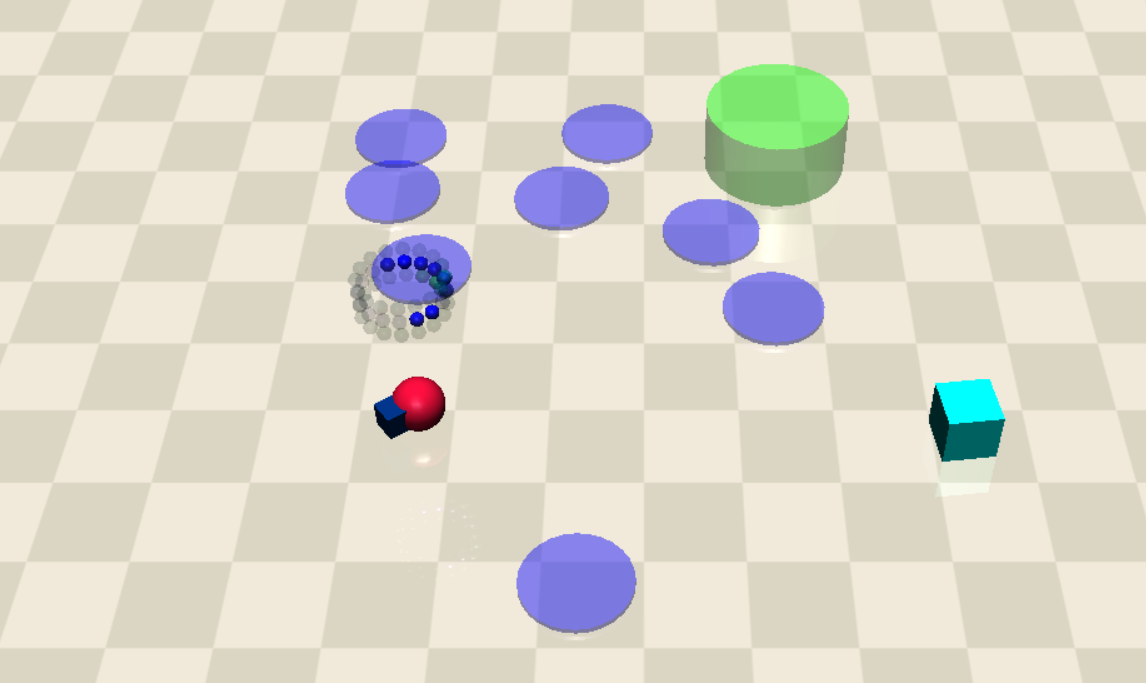
\includegraphics [width=0.4\textwidth, height=0.25\textwidth]{images/goal.png}}
    \subfloat[Circle Task]{
            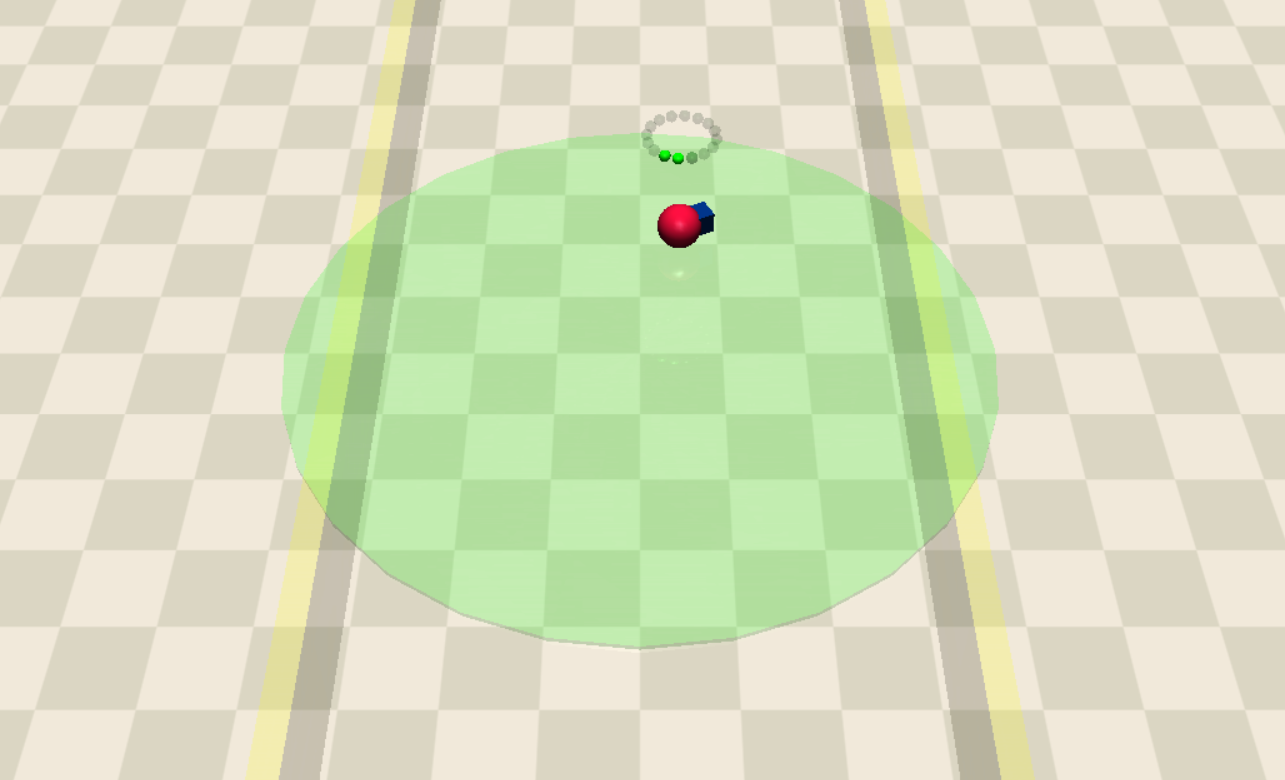
\includegraphics [width=0.4\textwidth, height=0.25\textwidth]{images/circle.png}}
    \\
    \subfloat[Push Task]{
            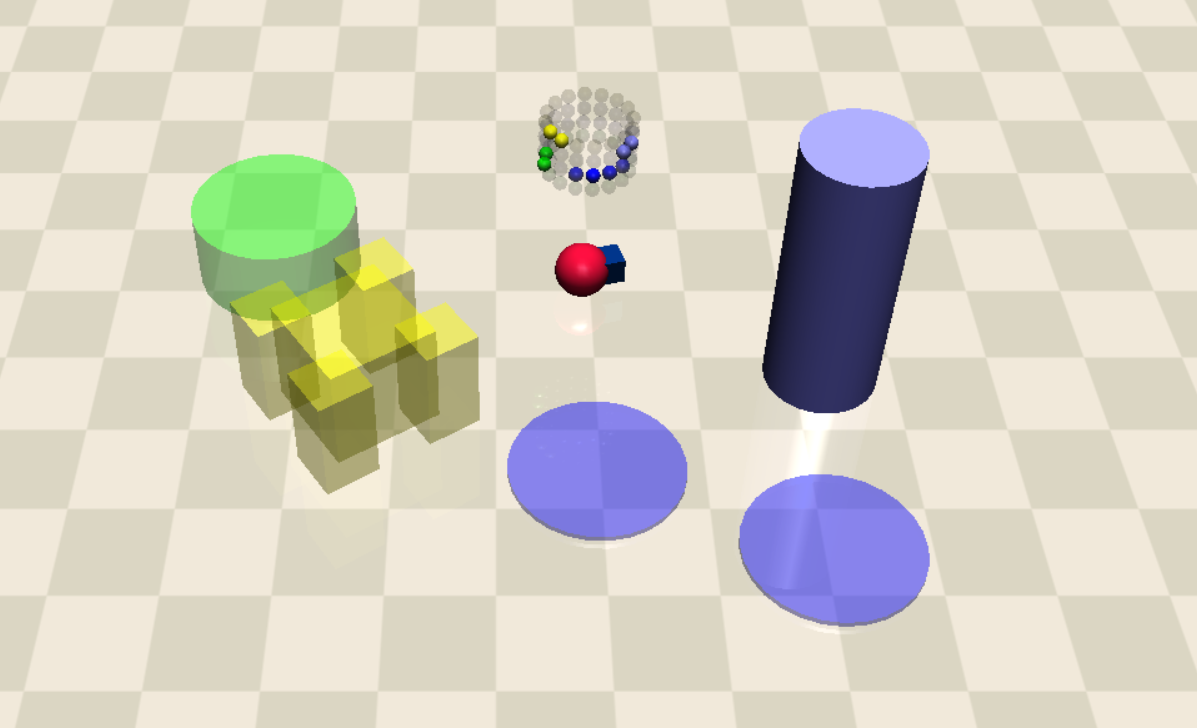
\includegraphics [width=0.4\textwidth, height=0.25\textwidth]{images/push.png}}
    \subfloat[MultiGoal Task]{
            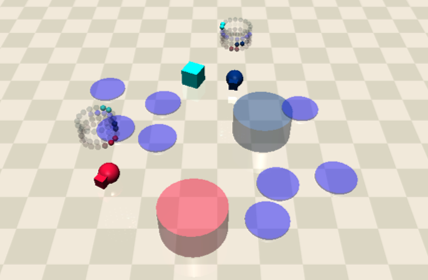
\includegraphics [width=0.4\textwidth, height=0.25\textwidth]{images/multiGoal.png}}
    \caption{不同任务场景图}
    \end{figure}

\subsection{安全可达空间实验}
为刻画机器人在不确定环境中的可行运动范围，本文基于包含智能体状态及环境观测的离线数据，对系统进行可达性分析预训练，从而构建机器人的安全可达空间。该安全空间用于刻画在给定动力学约束和环境条件下，系统状态是否能够在未来演化过程中满足安全约束，为后续在线决策提供安全判据。

通过对离线数据进行可达性分析，可以在状态空间中学习得到一类安全值函数，从而衡量不同状态的安全程度。如图 ~\ref{fig:safety_space} 所示，其中蓝色标记的区域表示安全值大于 0，说明系统在该区域内存在潜在的安全风险，即危险区域；其余区域则对应安全值小于等于 0，被视为满足安全约束的安全区域。该分布结果表明，可达性分析能够有效区分安全与非安全状态，为后续安全控制提供明确的边界信息。

此外，当改变机器人速度的大小与运动方向时，可以观察到安全域分布的显著变化。表明，安全可达空间与机器人的运动状态的相关性。当智能体速度增大或朝向发生变化时，其在有限时间内的可达集合随之改变，安全域边界也会发生调整。

上述结果表明，基于可达性分析构建的安全空间能够较好地反映环境风险与运动状态之间的关系。将该安全空间作为先验信息引入后续策略学习过程，有助于强化学习策略在在线决策时获得更明确的安全约束参考。
\begin{figure*}[thpb]
	\centering
	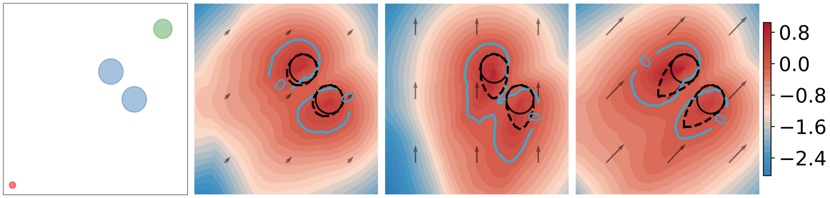
\includegraphics[width=\textwidth]{images/safe_space.png}
	\caption{安全空间分布图。蓝色曲线所包围的区域（安全值 > 0）表示危险区域，其余区域为安全区域。安全域会随着输入速度和方向的变化而发生改变。}
	\label{fig:safety_space}
\end{figure*}

\subsection{对比实验}
为评估完整框架在安全性与任务性能上的综合表现，本文在 Safety-Gymnasium 的 Goal、Circle、Push 与 MultiGoal 任务中与其他基准算法进行对比。

\subsubsection{基线方法}
本文在单智能体和多智能体场景中，与多种经典的安全强化学习算法进行对比，包括 PPO~\cite{schulman2017ppo}、 PCPO~\cite{yang2020projection} 、 PPO-Lag~\cite{stooke2020responsive} 、 TRPO-Lag~\cite{achiam2017cpo} ，多智能体实验包含了 MAPPO 、 HAPPO~\cite{kuba2022happo} 、 MACPO 以及 MAPPO\_Lag。

需要注意的是，ATACOM~\cite{liu2022atacom} 需要任务特定的约束雅可比矩阵以及扩展动作空间，因此在 Safety-Gymnasium 基准环境上进行直接比较较为困难；相比之下，本文的方法采用一种基于距离的简化安全过滤器，用于在点机器人任务中近似实现流形投影。

\subsubsection{评估指标与实现细节}

\begin{itemize}
\item \textbf{Reward}：每个回合的累计奖励（越高越好）。
\item \textbf{Cost}：累计约束违反次数（越低越好，理想值为 0）。
\item \textbf{Steps}：回合长度（直到到达目标或达到时间上限的步数）。
\end{itemize}

表~\ref{tab:hyperparams} 总结了实验中的关键超参数。所有实验均以 PPO~\cite{schulman2017ppo} 作为基础强化学习算法。表~\ref{tab:main_results} 和表~\ref{tab:ablation} 中的每个配置均在 3 个随机种子下训练 $10^5$ 个时间步；表~\ref{tab:ekf_comparison} 使用 5 个随机种子。基线方法报告平均性能，而 CMPL 报告 mean ± std。

\begin{table}[t]
\centering
\caption{实验超参数设置}
\label{tab:hyperparams}
\resizebox{0.8\columnwidth}{!}{
\begin{tabular}{ll|ll}
\toprule
\multicolumn{2}{c|}{\textbf{PPO 与训练参数}} & \multicolumn{2}{c}{\textbf{安全过滤器与 EKF}} \\
\midrule
学习率 & $3 \times 10^{-4}$ & 基础危险半径 $d_0$ & 0.6,m \\
折扣因子 $\gamma$ & 0.99 & 停止半径 $d_{\text{stop}}$ & 0.3,m \\
GAE 参数 $\lambda$ & 0.95 & 危险区域半径 $d_{\text{hazard}}$ & 0.2,m \\
网络结构 & MLP(256, 256) & 奖励校准权重 $\lambda$ & 0.1 \\
Rollout 缓冲区 & 2048 步 & 修正增益 $K_c$ & 10.0 \\
训练步数 & $10^5$ & EKF 窗口长度 $L$ & 10 \\
评估回合数 & 50 & CNN 架构 & Conv1d $\rightarrow$ FC \\
随机种子 (表 I,III / IV) & 3 / 5 & CNN 参数量 & $\sim$5K \\
Batch size (PPO) & 64 & 预训练轮数 & 100 \\
Clip ratio $\epsilon$ & 0.2 & 安全裕度参数 $\eta$ / $\delta$ & 0.1,m / 1.0 \\
&  & 噪声参数 $\sigma_{\text{base}}$ / $k$ & 0.1,m / 5.0 \\
\bottomrule
\end{tabular}
}
\end{table}

% 为系统性验证所提出约束流形方法在安全关键任务中的有效性，本文在 Safe-Policy-Optimization（SafePO）（Ji 等人，2023）实验平台上进行了广泛评估，并与多种代表性的安全强化学习方法进行了对比实验。SafePO 平台提供了标准化的安全强化学习基准任务与评估接口，能够较为全面地反映不同算法在安全性与性能之间的权衡能力。

% 本文选用累计奖励（Reward）和累计成本（Cost）作为主要评估指标，其中成本值越低表示策略越安全。考虑到机器人系统通常属于安全关键型应用场景，本文在实验评估中将安全性作为首要指标，在满足安全约束的前提下进一步追求更高的任务回报。为增强不同方法在安全维度上的区分度，并突出安全约束的重要性，本文对 SafePO 中的原始奖励函数进行了改造，引入了不同强度的碰撞惩罚项，并系统分析了碰撞惩罚强度变化对各类方法性能的影响。

\subsubsection{实验结果}
实验结果汇总于表~\ref{tab:main_results} 中。
本文的方法（CMPL）在所有任务和惩罚设置下都取得了最低的代价（cost），表明该方法对惩罚参数调节具有很强的鲁棒性。相比之下，基线方法对惩罚系数非常敏感。例如，在 Goal 任务中，PPO-Lag 的 cost 从 5.46（$r_{\text{col}}=0.1$）变化到 13.91（$r_{\text{col}}=0.5$），波动达到 $2.5\times$。
在 Circle 和 Push 任务中，基线方法仍表现出较明显的约束违背，cost 大致分布在 5-38 之间；相比之下，CMPL 的 cost 始终维持在较低水平，Circle 任务为 1.38-1.55，Push 任务为 0.92-1.23。可以看到，当碰撞惩罚降低至 $r_{\text{col}}=0.1$ 时，cost 有小幅上升。其原因在于，较低的碰撞惩罚会使强化学习策略更倾向于选择激进探索动作，这类动作虽然可能提高短期任务收益，但也会给安全过滤器带来更大的修正压力。

从回合长度来看，CMPL 在不同 $r_{\text{col}}$ 设置下变化较小，例如 Goal 任务基本保持在 350 步左右。这一现象与安全过滤机制有关：当机器人接近障碍物时，安全过滤器会对动作进行修正并限制其运动速度，而该过程并不依赖奖励函数中的碰撞惩罚系数。相较而言，部分基线方法在低惩罚设置下更容易选择距离障碍物较近的路径，甚至以更高风险换取更短的到达时间，因此回合长度会出现下降。需要注意的是，CMPL 在维持低约束违背的同时，并未明显牺牲任务收益，在 Goal 和 Push 任务中仍取得较高奖励，说明约束流形过滤机制能够在安全性和任务性能之间保持较好的协调。

在包含两个智能体的 Multi-Goal 任务中，约束违背主要来自智能体之间的相互碰撞以及智能体与障碍物之间的碰撞。由于多智能体场景中的交互关系更加复杂，所有基线方法的 cost 均处于较高水平，约为 $12.48$-$36.13$。CMPL 则将 cost 降至 $0.07$，同时仍保持正向奖励。该结果说明，本文提出的约束流形安全过滤方法并不局限于单智能体避障任务，也可以扩展到多智能体场景中，用于同时处理静态障碍物避让和智能体间避碰问题。
\begin{table*}[h!]
    \begin{center}
      \caption{Safety-Gymnasium 在不同任务和惩罚系数设置下的结果}
      \label{tab:main_results}
      \resizebox{\textwidth}{26mm}{
      \begin{tabular}{cc|*{4}{ccc|}ccc} \hline
      \multicolumn{2}{c|}{Algorithm} &
      \multicolumn{3}{c|}{PPO} &
      \multicolumn{3}{c|}{PCPO} &
      \multicolumn{3}{c|}{PPO\_Lag} &
      \multicolumn{3}{c|}{TRPO\_Lag} &
      \multicolumn{3}{c}{CMPL}\\
      TASK & $r_{collision}$
          & reward & cost & step
          & reward & cost & step
          & reward & cost & step
          & reward & cost & step
          & reward & cost & step \\ \hline

      \multirow{3}{*}{GOAL}
      & 1
          & -6.87 &  7.77 & 516
          & -2.11 &  3.75 & 342
          & -9.67 & 10.00 & 713
          & -3.08 &  4.01 & 490
          &  \textcolor{red}{1.68}{\tiny$\pm$0.3} &  \textcolor{Green3}{\textbf{0.00}} & 352{\tiny$\pm$18} \\
      & 0.5
          & -2.71 &  8.45 & 335
          & -0.71 &  4.66 & 252
          & -5.91 & 13.91 & 505
          &  0.00 &  3.53 & 226
          &  \textcolor{red}{1.72}{\tiny$\pm$0.4} &  \textcolor{Green3}{\textbf{0.00}} & 348{\tiny$\pm$21} \\
      & 0.1
          & 1.59 & 4.88 & 101
          & 1.65 & 3.94 & 101
          & 1.50 & 5.46 & 119
          & \textcolor{red}{1.79} & 3.01 & 84
          & 1.69{\tiny$\pm$0.3} & \textcolor{Green3}{\textbf{0.00}} & 352{\tiny$\pm$19} \\ \hline

      \multirow{3}{*}{CIRCLE}
      & 1
          & 5.88 & 5.49 & 500
          & 30.36 & 2.64 & 500
          & 8.14 & 6.82 & 500
          & \textcolor{red}{34.61} & 2.13 & 500
          & 16.42{\tiny$\pm$1.8} & \textcolor{Green3}{1.38}{\tiny$\pm$0.5} & 500 \\
      & 0.5
          & 23.24 & 8.51 & 500
          & 31.32 & 3.24 & 500
          & \textcolor{red}{33.67} & 5.00 & 500
          & 32.68 & 4.78 & 500
          & 17.05{\tiny$\pm$2.1} & \textcolor{Green3}{1.42}{\tiny$\pm$0.6} & 500 \\
      & 0.1
          & \textcolor{red}{38.32} & 31.83 & 500
          & 34.47 & 15.59 & 500
          & 37.14 & 23.98 & 500
          & 36.91 & 38.13 & 500
          & 18.23{\tiny$\pm$2.4} & \textcolor{Green3}{1.55}{\tiny$\pm$0.7} & 500 \\ \hline

      \multirow{3}{*}{PUSH}
      & 1
          & -10.43 & 9.99 & 996
          & -5.02 & 4.88 & 986
          & -8.71 & 8.52 & 992
          & -2.76 & 2.89 & 978
          &  \textcolor{red}{0.38}{\tiny$\pm$0.4} & \textcolor{Green3}{0.92}{\tiny$\pm$0.4} & 995{\tiny$\pm$3} \\
      & 0.5
          & -4.13 & 8.45 & 990
          & -3.30 & 6.50 & 989
          & -5.27 & 9.31 & 993
          & -2.99 & 6.49 & 967
          & \textcolor{red}{0.51}{\tiny$\pm$0.5} & \textcolor{Green3}{1.07}{\tiny$\pm$0.5} & 997{\tiny$\pm$2} \\
      & 0.1
          & -1.50 & 18.31 & 977
          & -0.74 & 11.93 & 947
          & -1.09 & 14.88 & 969
          & -1.10 & 13.28 & 978
          & \textcolor{red}{0.67}{\tiny$\pm$0.5} & \textcolor{Green3}{1.23}{\tiny$\pm$0.6} & 998{\tiny$\pm$2} \\ \hline

      \multicolumn{2}{c|}{Algorithm} &
      \multicolumn{3}{c|}{MAPPO} &
      \multicolumn{3}{c|}{HAPPO} &
      \multicolumn{3}{c|}{MACPO} &
      \multicolumn{3}{c|}{MAPPO\_Lag} &
      \multicolumn{3}{c}{CMPL}\\
      TASK & $r_{collision}$
          & reward & cost & step
          & reward & cost & step
          & reward & cost & step
          & reward & cost & step
          & reward & cost & step \\ \hline

      MULTI\_GOAL
      & 1
          & -23.42 & 23.12 & 362
          & -17.75 & 17.64 & 199
          & -36.41 & 36.13 & 182
          & -13.50 & 12.48 & 192
          & \textcolor{red}{0.01}{\tiny$\pm$0.2} & \textcolor{Green3}{0.07}{\tiny$\pm$0.1} & 346{\tiny$\pm$15}
  \\ \hline

      \end{tabular}
      }
    \end{center}
  \end{table*}
\subsection{消融实验}
在单智能体导航避障任务中，为更真实地刻画实际机器人在感知与定位过程中面临的不确定性，本文通过在环境中引入随机噪声来模拟传感器误差。
采用 PPO 算法作为基础强化学习方法，通过在 PPO 基线方法上逐步加入各个模块，
验证每个组件的贡献。实验结果为 3 个随机种子、$10^5$ 训练步以及 50 个评估回合的平均值。完整系统在速度相关传感器噪声条件下运行（$\sigma_{\text{base}} = 0.1$m，$k=5$）（见表~\ref{tab:ablation}）。
\begin{table}[t]
\centering
\caption{Goal 任务消融实验结果}
\label{tab:ablation}
\begin{tabular}{l|cc}
\toprule
配置 & Reward & Cost \\
\midrule
PPO（baseline） & $19.08 \pm 4.93$ & $64.59 \pm 8.51$ \\
+流形过滤器 & $12.20 \pm 5.06$ & $38.22 \pm 13.61$ \\
+可达性预训练 & $-8.44 \pm 8.21$ & $18.97 \pm 9.00$ \\
+EKF（完整系统，含噪声） & $-4.32 \pm 3.68$ & $\mathbf{12.51 \pm 6.32}$ \\
  \midrule
  完整系统（无奖励校准） & $16.83 \pm 0.92$ & $71.63 \pm 10.02$ \\
  \bottomrule
  \end{tabular}
  \end{table}

\begin{figure}[t]
\centering

\includegraphics[width=\linewidth]{images/training_curves.png}
\caption{学习曲线体现各组件的贡献。(a) 不同配置下的回合奖励；(b) 回合 cost（安全违规次数）}
\label{fig:training_curves}
\end{figure}

图~\ref{fig:training_curves} 展示了各配置的训练曲线。结果表明，每个组件都对整体性能产生了重要贡献：
\begin{itemize}
\item \textbf{流形过滤器（Manifold Filter）}：通过零空间投影（null-space projection）将 cost 降低了 41\%（$64.59 \rightarrow 38.22$），但由于不安全动作被修正，reward 有一定下降。

\item \textbf{可达性预训练（Reachability Pretraining）}：通过将策略约束在可行区域 $\mathcal{S}^*_f$ 内，并引入更大的安全裕度，使 cost 相比基线进一步降低了 71\%（$64.59 \rightarrow 18.97$）。

\item \textbf{数据驱动 EKF}：即使在速度相关的传感器噪声存在的情况下，仍然能够保持相近的安全性（$12.51$），说明该方法在感知不确定性下依然能够稳健地执行约束。

\item \textbf{奖励校准（Reward Calibration）}：对安全性至关重要——如果移除该机制，智能体会利用约束边界来获得更高奖励（$16.83$），但同时会产生显著更多的违规（$71.63$ 对比 $12.51$）。
\end{itemize}

\subsection{EKF 对比实验}
为了单独评估 EKF 的贡献，首先在无噪声条件下训练一个带安全过滤器的单智能体策略，然后在部署阶段引入速度相关噪声~\eqref{eq:vel_noise}（$\sigma_{\text{base}} = 0.1$m，$k = 5$），并比较三种状态估计配置。表~\ref{tab:ekf_comparison} 给出了在 5 个随机种子和 50 个评估回合上的平均结果。

\begin{table}[t]
\centering
\caption{Goal 任务 EKF 对比实验}
\label{tab:ekf_comparison}
\resizebox{0.8\columnwidth}{!}{
\begin{tabular}{l|ccc}
\toprule
方法 & 位置误差 (m) & Reward & Cost \\
\midrule
原始 GPS & $0.54 {\pm} 0.18$ & $-7.92 {\pm} 1.43$ & $9.14 {\pm} 2.37$ \\
EKF（固定 $R$） & $0.41 {\pm} 0.13$ & $-7.86 {\pm} 1.21$ & $9.58 {\pm} 2.15$ \\
EKF（学习得到的 $R$） & $\mathbf{0.27 {\pm} 0.05}$ & $-7.87 {\pm} 0.94$ & $\mathbf{9.31 {\pm} 1.68}$ \\
\bottomrule
\end{tabular}
}
\end{table}

采用学习得到协方差矩阵的 EKF 在位置精度方面表现最佳（$0.27$m），相比原始 GPS 将误差降低了 49\%，相比固定 $R$ 的 EKF 降低了 34\%。同时，其误差方差也显著降低，为原始 GPS 的约 $1/3.6$（$0.05$ 对比 $0.18$）。

虽然在这一独立评估中各方法的 cost 差异不大，但消融实验（表~\ref{tab:ablation}）展示了完整系统的优势：在包含传感器噪声的训练条件下，cost 从 $18.97$ 进一步降低到 $12.51$。

\textbf{计算开销。} NoiseAdapter CNN 带来的计算开销非常小：该网络约有 5K 个参数，在 CPU 上每一步推理时间小于 $0.1$,ms，相比环境步进时间（5ms）和 PPO 前向传播时间（1ms）几乎可以忽略不计。

预训练阶段需要进行 30 次随机探索回合（约 2 分钟）以及 100 个 epoch 的负对数似然（NLL）优化（约 30 秒），这是一次性的开销，可以在整个训练过程中被摊销。

实验表明，该 CNN 在约 50 个 epoch 内即可收敛（损失在约 $-3.7$ 处进入平台期）。学习得到的 $R_t$ 能够实现平滑自适应：在高速运动时预测较大的测量噪声协方差，在低速运动时预测较小的协方差，这与理论上的速度—噪声模型~\eqref{eq:vel_noise} 相一致。

\subsection{Webots 仿真实验}
本文在 Webots~\cite{webots2004} 仿真环境中的 E-puck 机器人上验证了安全过滤器和 EKF 的有效性。为了测试方法对控制策略的策略无关迁移能力（policy-agnostic transferability），实验中刻意使用 P 控制器（而非强化学习策略）进行控制。

通过 ROS 2 验证了系统部署，使用 webots\_ros2\_driver 进行仿真接口集成，其中安全过滤器作为独立的 ROS2 节点运行（见图~\ref{fig:ros2arch}）。
\begin{figure}[t]
\centering

\includegraphics[width=\columnwidth]{images/ros_architecture.png}
\caption{ROS2 集成架构}
\label{fig:ros2arch}
\end{figure}

为了验证安全层具有策略无关性（policy-agnostic），本文在 E-puck 机器人（直径 $\varnothing70mm$）上部署了基于距离的安全过滤器和标准 EKF（固定 $R$），并在 Webots 仿真环境中进行实验。实验场景为一个 $2\text{m} \times 2\text{m}$ 的区域，其中放置 6 个圆柱形障碍物，GPS 噪声为 $\sigma=0.04$m，IMU 航向角噪声为 $\sigma=0.05$,rad。名义控制策略刻意采用一个简单的 P 控制器——而不是训练得到的强化学习策略——以证明该安全架构可以在无需重新训练的情况下迁移到新的机器人平台和控制器上。

在 Webots 实验中，安全过滤器采用基于距离的速度缩放机制（相比流形过滤器更为简单），同时使用具有固定噪声协方差的标准 EKF。实验结果如图~\ref{fig:ros}，在没有安全过滤的情况下，20 次实验中有 8 次发生碰撞（碰撞率 40\%），其中 4 次由于碰撞导致导航错误而未能到达目标（成功率 80\%）。而本文的方法实现了零碰撞，成功率达到 85\%。其中 3 次失败是由于机器人在密集障碍区域附近发生导航超时，但均在没有碰撞的情况下安全结束。值得注意的是，安全过滤器实际上提高了成功率（85\% 对比 80\%），因为未过滤的碰撞会破坏导航稳定性。EKF 通过融合里程计和 GPS 测量，将位置误差降低了 27\%（$0.051 \rightarrow 0.037$m）（见表~\ref{tab:webots}）。

\begin{table}[t]
\centering
\caption{Webots E-puck 实验验证}
\label{tab:webots}
\begin{tabular}{l|cc}
\toprule
指标 & 无过滤 & \textbf{本文方法（完整系统）} \\
\midrule
成功率 (\%) & 80.0 & $\mathbf{85.0}$ \\
碰撞率 (\%) & 40.0 & $\mathbf{0.0}$ \\
位置误差 (m) & $0.051 \pm 0.001$ & $\mathbf{0.037 \pm 0.001}$ \\
路径长度 (m) & $\mathbf{0.94 \pm 0.41}$ & $1.80 \pm 1.49$ \\
\bottomrule
\end{tabular}
\end{table}

\begin{figure*}[t]
\centering
\subfloat[实验环境]{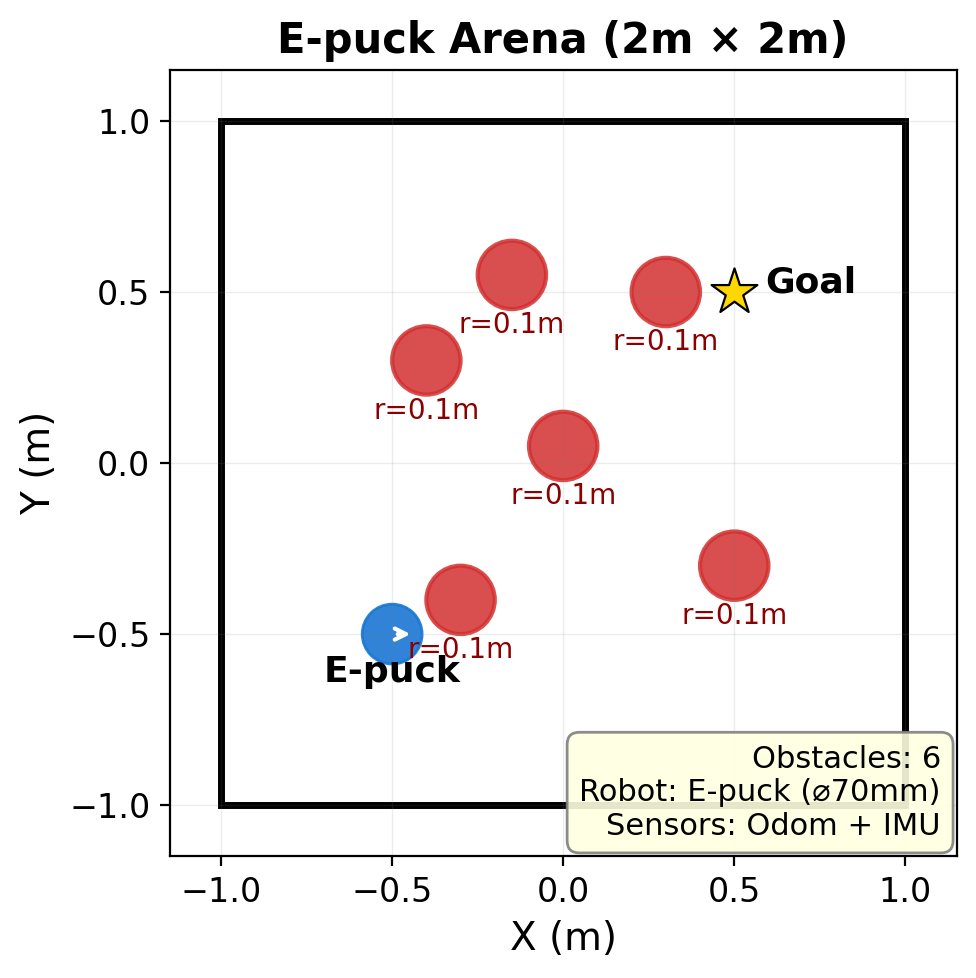
\includegraphics[height=4cm]{images/ros_setup.png}}
\hfill
\subfloat[轨迹对比]{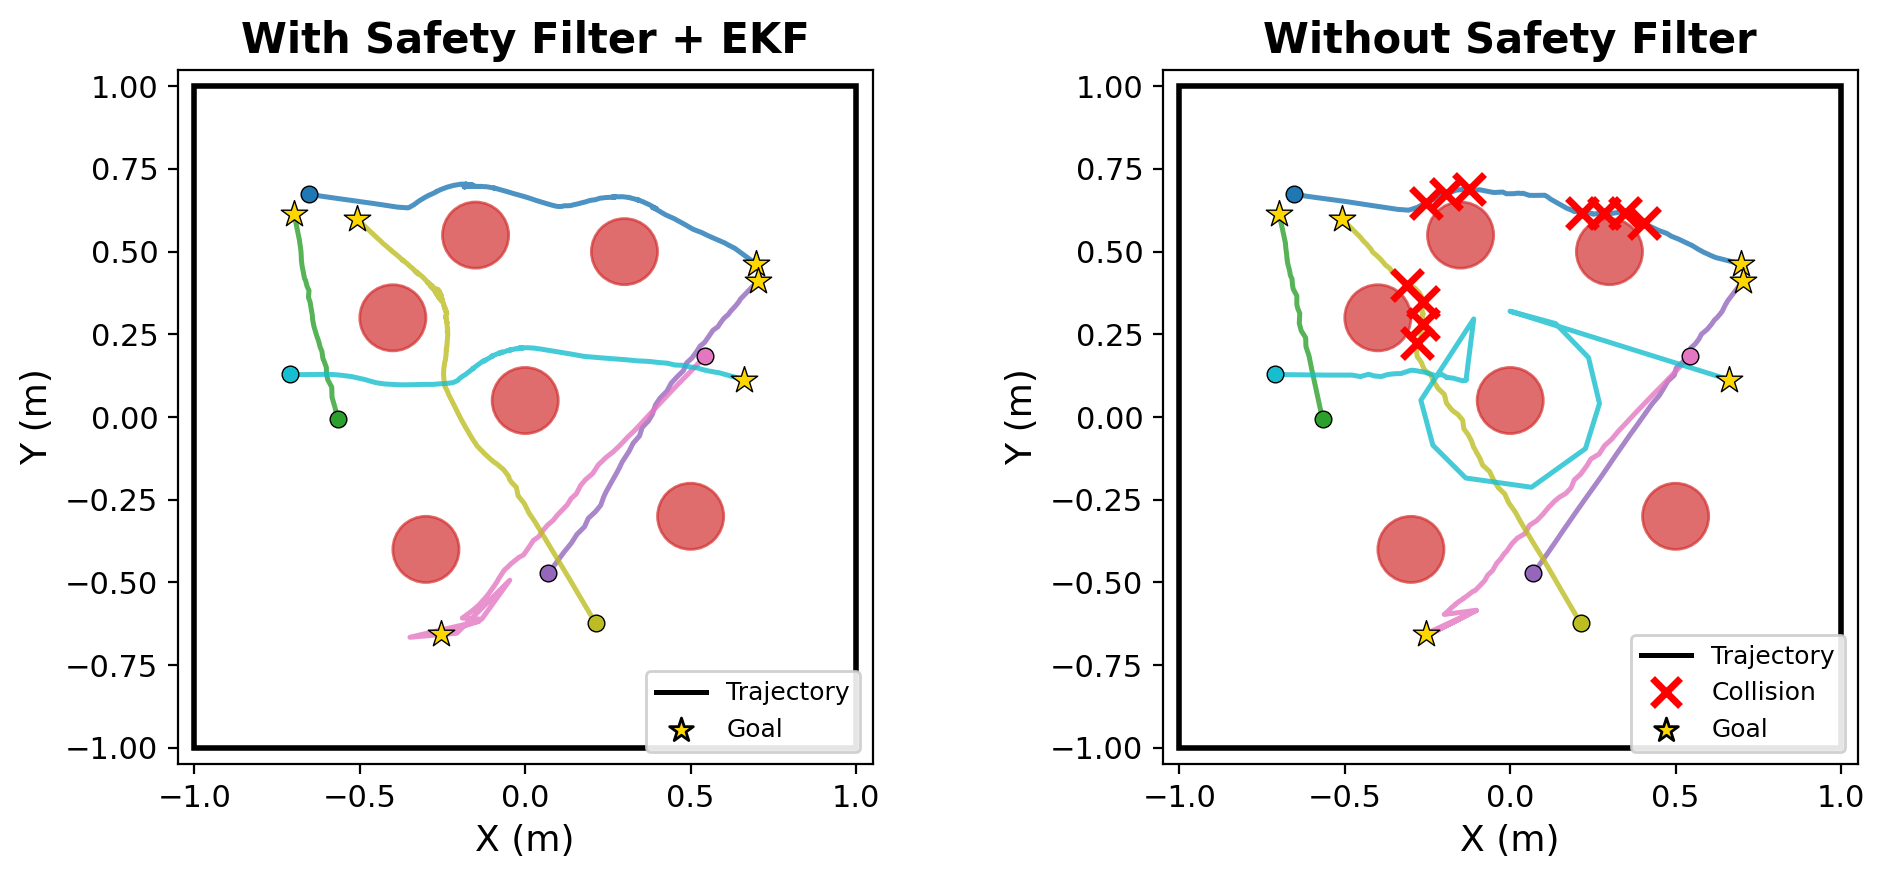
\includegraphics[height=4cm]{images/trajectory.png}}
\caption{Webots 中 E-puck 实验验证。(a) 含 6 个障碍物的实验环境。(b) 轨迹对比：带安全过滤器 + EKF（左）与无过滤（右，$\times$ 表示碰撞）。}
\label{fig:ros}
\end{figure*}



% \subsection{ROS平台验证实验}

% 为进一步验证所提出安全强化学习框架在实际机器人系统中的可行性与工程适用性，本文将该方法部署至 ROS 平台，并在 Webots 仿真环境中开展导航避障实验。实验对象选用 E-puck 移动机器人模型，通过其搭载的 IMU 传感器获取运动状态信息，并结合所提出的数据驱动定位算法，实现对机器人位姿的在线估计与更新。
% \begin{figure}
%     \centering
%     
\includegraphics[width=1\linewidth]{images/ros_architecture.png}
%     \caption{ros architecture}
%     \label{fig:placeholder}
% \end{figure}
% 在实验过程中，机器人在包含静态障碍物的环境中执行自主导航任务，目标是在满足安全约束的前提下，从初始位置安全到达指定目标点。系统通过 ROS 框架完成传感器数据的采集、状态估计、策略推理以及控制指令的发布，同时利用 rviz 可视化工具对机器人运动轨迹进行实时显示与分析。实验结果如图 4(b) 所示，其中蓝色轨迹表示 Webots 仿真环境中机器人的真实运动轨迹，红色轨迹表示由所提出的数据驱动定位算法估计得到的轨迹。

% 从实验结果可以看出，红色估计轨迹与真实轨迹整体保持较高的一致性，表明所提出的定位方法能够在存在传感器噪声的情况下较为准确地估计机器人位姿。同时，在策略执行过程中，机器人能够有效避开环境中的障碍物，并在未发生安全约束违规的情况下顺利到达目标位置，验证了所提出安全策略在实际控制回路中的有效性与稳定性。

% 上述 ROS 平台与 Webots 仿真环境下的实验结果表明，本文提出的安全强化学习框架不仅在理论和仿真层面具有良好性能，同时具备较强的工程实现能力，为未来向真实机器人系统的迁移与应用奠定了坚实基础。

% \begin{figure}[thpb]
% \centering
% %\includegraphics[width=3in]{fig5}
% \subfloat[Experimental Scenario]{
% 		
\includegraphics [width=0.4\textwidth, height=0.4\textwidth]{任务1-MICL-2023-ConstrainedMARL-ConstrainedfactorSLAM/IROS/ROS.png}}
% \subfloat[Robot Trajectory]{
% 		
\includegraphics [width=0.4\textwidth, height=0.4\textwidth]{任务1-MICL-2023-ConstrainedMARL-ConstrainedfactorSLAM/IROS/轨迹.jpg}}
% \caption{ROS Platform Verification Experiment}
% \end{figure}

\section{本章小结}

本章围绕安全强化学习在机器人导航避障问题，构建了安全可达空间刻画 + 策略生成 + 安全过滤 + 状态估计的CMPL框架。
针对强化学习策略在复杂场景下可能出现的约束违规风险，本文首先根据系统约束构建安全可达空间，为在线决策提供风险边界，
并进一步从约束流形视角设计了安全过滤机制，
通过对名义动作进行在线修正，在不改变上层策略结构的前提下实现对安全约束的显式满足，并给出了相应的稳定性分析。

同时，为提升系统在噪声感知条件下的可用性，本章结合运动学模型与多源传感信息，构建了 EKF 状态估计模块，
并进一步引入基于数据驱动的观测噪声自适应建模，以增强定位精度与鲁棒性。
仿真实验结果表明，CMPL 在不同任务和控制策略下均能降低碰撞风险，并保持较好的任务表现。
上述工作为后续多机器人编队场景中的安全协同控制研究提供了方法基础。
